\documentclass[a0,portrait]{a0poster}

\usepackage{multicol} % This is so we can have multiple columns of text side-by-side
\columnsep=100pt % This is the amount of white space between the columns in the poster
\columnseprule=3pt % This is the thickness of the black line between the columns in the poster

\usepackage[svgnames]{xcolor} % Specify colors by their 'svgnames', for a full list of all colors available see here: http://www.latextemplates.com/svgnames-colors

\usepackage{graphicx} % Required for including images
\graphicspath{{figures/}} % Location of the graphics files
\usepackage{booktabs} % Top and bottom rules for table
\usepackage[font=small,labelfont=bf]{caption} % Required for specifying captions to tables and figures
\usepackage{amsfonts, amsmath, amsthm, amssymb} % For math fonts, symbols and environments
\usepackage{wrapfig} % Allows wrapping text around tables and figures
\usepackage[utf8x]{inputenc}

\begin{document}

\begin{minipage}[b]{0.75\linewidth}
\veryHuge \textbf{Transportation model and value
creation:} \color{Black}\\ % Title
\Huge\textit{ A multicriteria decision
analysis approach}\\[2cm] % Subtitle
\huge \textbf{Marco Repetto}\\[0.5cm] % Author(s)
\huge Università degli Studi di Milano\\[0.4cm] % University/organization
\Large Faculty of Political, Economic and Social Sciences\\[0.4cm]
\Large \texttt{marco.repetto@studenti.unimi.it}\\
\end{minipage}
%
\begin{minipage}[b]{0.25\linewidth}

\includegraphics[width=20cm]{logo}\\
\end{minipage}

\vspace{1cm} % A bit of extra white space between the header and poster content

\begin{multicols}{2} % This is how many columns your poster will be broken into, a portrait poster is generally split into 2 columns

\color{Navy} % Navy color for the abstract

\begin{abstract}
In the poster is proposed a review of the multicriteria decision analysis tool with particular attention on the Goal Programming approach. In order to show its potential two practical cases are taken into account. In the first case is solved a problem of optimal income allocation between multinational entities under several constraints derived from the field of transfer pricing. In the second case the problem is stated as an optimization of the goods/trash flow in a Green Supply Chain network involving a closed loop setting. Both the cases used weights to identify the propensity of the decision maker toward a certain choice, therefore in order to support such decision and avoid any possible mistake in evaluating them an Analytic Hierarchy Process is set.

\end{abstract}

\color{SaddleBrown} % SaddleBrown color for the introduction

\section*{Introduction}
Value and MNE were probably the pairs of elements that characterized the way business was done in the last centuries, and still, nowadays they are something that cannot be left aside when we talk about the business environment. Because of this interest, different disciplines were created; ranging from management to accounting and from supply chain to logistics (which has its roots in the military planning field). In this dissertation, the scope will be to apply a multi-objective approach, namely the GP in order to prove the effectiveness of such method and its different flavors in the hand of the DM. The two models presented deal with the transportation of some particular element of the firm in order to create additional value for it. 


\color{DarkSlateGray} % DarkSlateGray color for the rest of the content

\section*{Main Objectives}

A firm and especially a MNE may be seen as a network of enterprises intertwined between each other in order to exploit the synergies provided by such union, if the framework of logistics it's used is possible to discern the flow between two or more of such firms in three different aspects, namely:

\begin{itemize}
 \item Goods: this flow is the most tangible one and may involve the movement of products from the rear line (production plan) to the front line (retail stores);    
\item Information: this flow consists of all the information necessary for the network to work, a good example may be the information of the demand that has to move back to the production plan in order to be fulfilled;
\item Finance: usually the finance flow is, among the information flow the one that permits the day to day operations of the network entities and supports the goods flow; this role is usually undertaken by the headquarter or in more complex groups to ad-hoc financial institutions inside the multinational company. 
\end{itemize}
In this setting the goal of the decision maker is to minimize the cost of each and every different aspects achieving the goal as effectively as possible.

\section*{Materials and Methods}
Even if the practice of decision-making is old as man, academics tend to date the roots of modern MCDA in the early 60s, where the focus at the time was to find the most preferred solution, or generating an approximation to the entire efficient frontier\cite{Greco2016}.


\subsection*{Mathematical Section}

The multicriteria decision problem formulation is the following: 
$$
Min[f_1(x),f_2(x),...,f_k(x)] \quad i=1,...,k \quad where \quad k\geq2
$$
	

A solution to a MCP would be optimal if it'd respected the Pareto Efficient assumption, namely that no other feasible solution exists that is at least as good with respect to all objectives and strictly better with respect to at least one objective. Mathematically it means that $\left\{x_1,...x_k\right\}$ is a solution if $\not\exists \left\{x'_1,...x'_k\right\}$
such that:
	\[
	g(f_1(x),f_2(x),...,f_k(x)) \leq g(f_1(x'),f_2(x'),...,f_k(x')) \quad \forall n \quad \in  \left\{1...k\right\}
	\]

	From the field of MCDA belongs the GP, such approach allows the DM to consider simultaneously several conflicting objectives. The idea behind such method is very simple, and is based on distance minimization; this means that at each objective function is associated a deviation variable that has to be minimized in batch with the other deviation variables coming from the other objective functions. Such models may be represented algebraically as follows:

\begin{equation*}
\begin{aligned}
& \underset{n,p}{\text{minimize}}
& & a=h(n,p) \\
& \text{subject to}
& & f_q(x)+n_q-p_q=b_q \\
& & & x\in F \\
& & & n_q,p_q\geq 0 
\end{aligned}
\end{equation*}

GP is vastly applied in many sciences\cite{Tamiz1998}. Its origins are dated back to the 50s, firstly introduced by Abraham Charnes and William Cooper\cite{Charnes1955} with an article on the optimal estimation of executive compensation. In such approach, three main different categories have been identified, namely the LGP, the WGP and the CGP.
In particular, the WGP allows for direct trade-offs between all unwanted deviational variables by using weights. As a result, WGP is more flexible but as counter-effect it requires more computational power. The mathematical formulation is the following one:

\begin{equation*}
\begin{aligned}
& \underset{n,p}{\text{minimize}}
& & \sum_{q=1}^{Q}(\frac{u_q n_q}{k_q}+\frac{v_q n_q}{k_q}) \\
& \text{subject to}
& & f_q(x)+n_q-p_q=b_q, \; q=1,...Q \\
& & & x\in F \\
& & & n_q,p_q\geq 0, \; q=1,...,Q 
\end{aligned}
\end{equation*}

\section*{Results}
In calculating the priority vector of the two different occurrences modeled the Analytic Hierarchy Process\cite{Saaty1980} was used.

\begin{wrapfigure}{l}{0.15\textwidth}
\begin{tabular}{l l}
\toprule
\textbf{Criteria} & \textbf{Weight} \\
\midrule
Operation Costs & 0.16 \\a0poster.cls
Tax Burden & 0.30 \\
Functional Allocation & 0.54 \\
Total & \textit{1.00} \\
\bottomrule
\end{tabular}
\captionof{table}{\color{Green} First model priority vector}
\end{wrapfigure}

The allocation resulted in four main area, namely: Denmark as unique manufacturer, Portugal as principal in charge of the management and holder of the know-how and intellectual properties and ultimately Cyprus and India as mere distributors.
\\
\\
\\
\begin{center}\vspace{1cm}
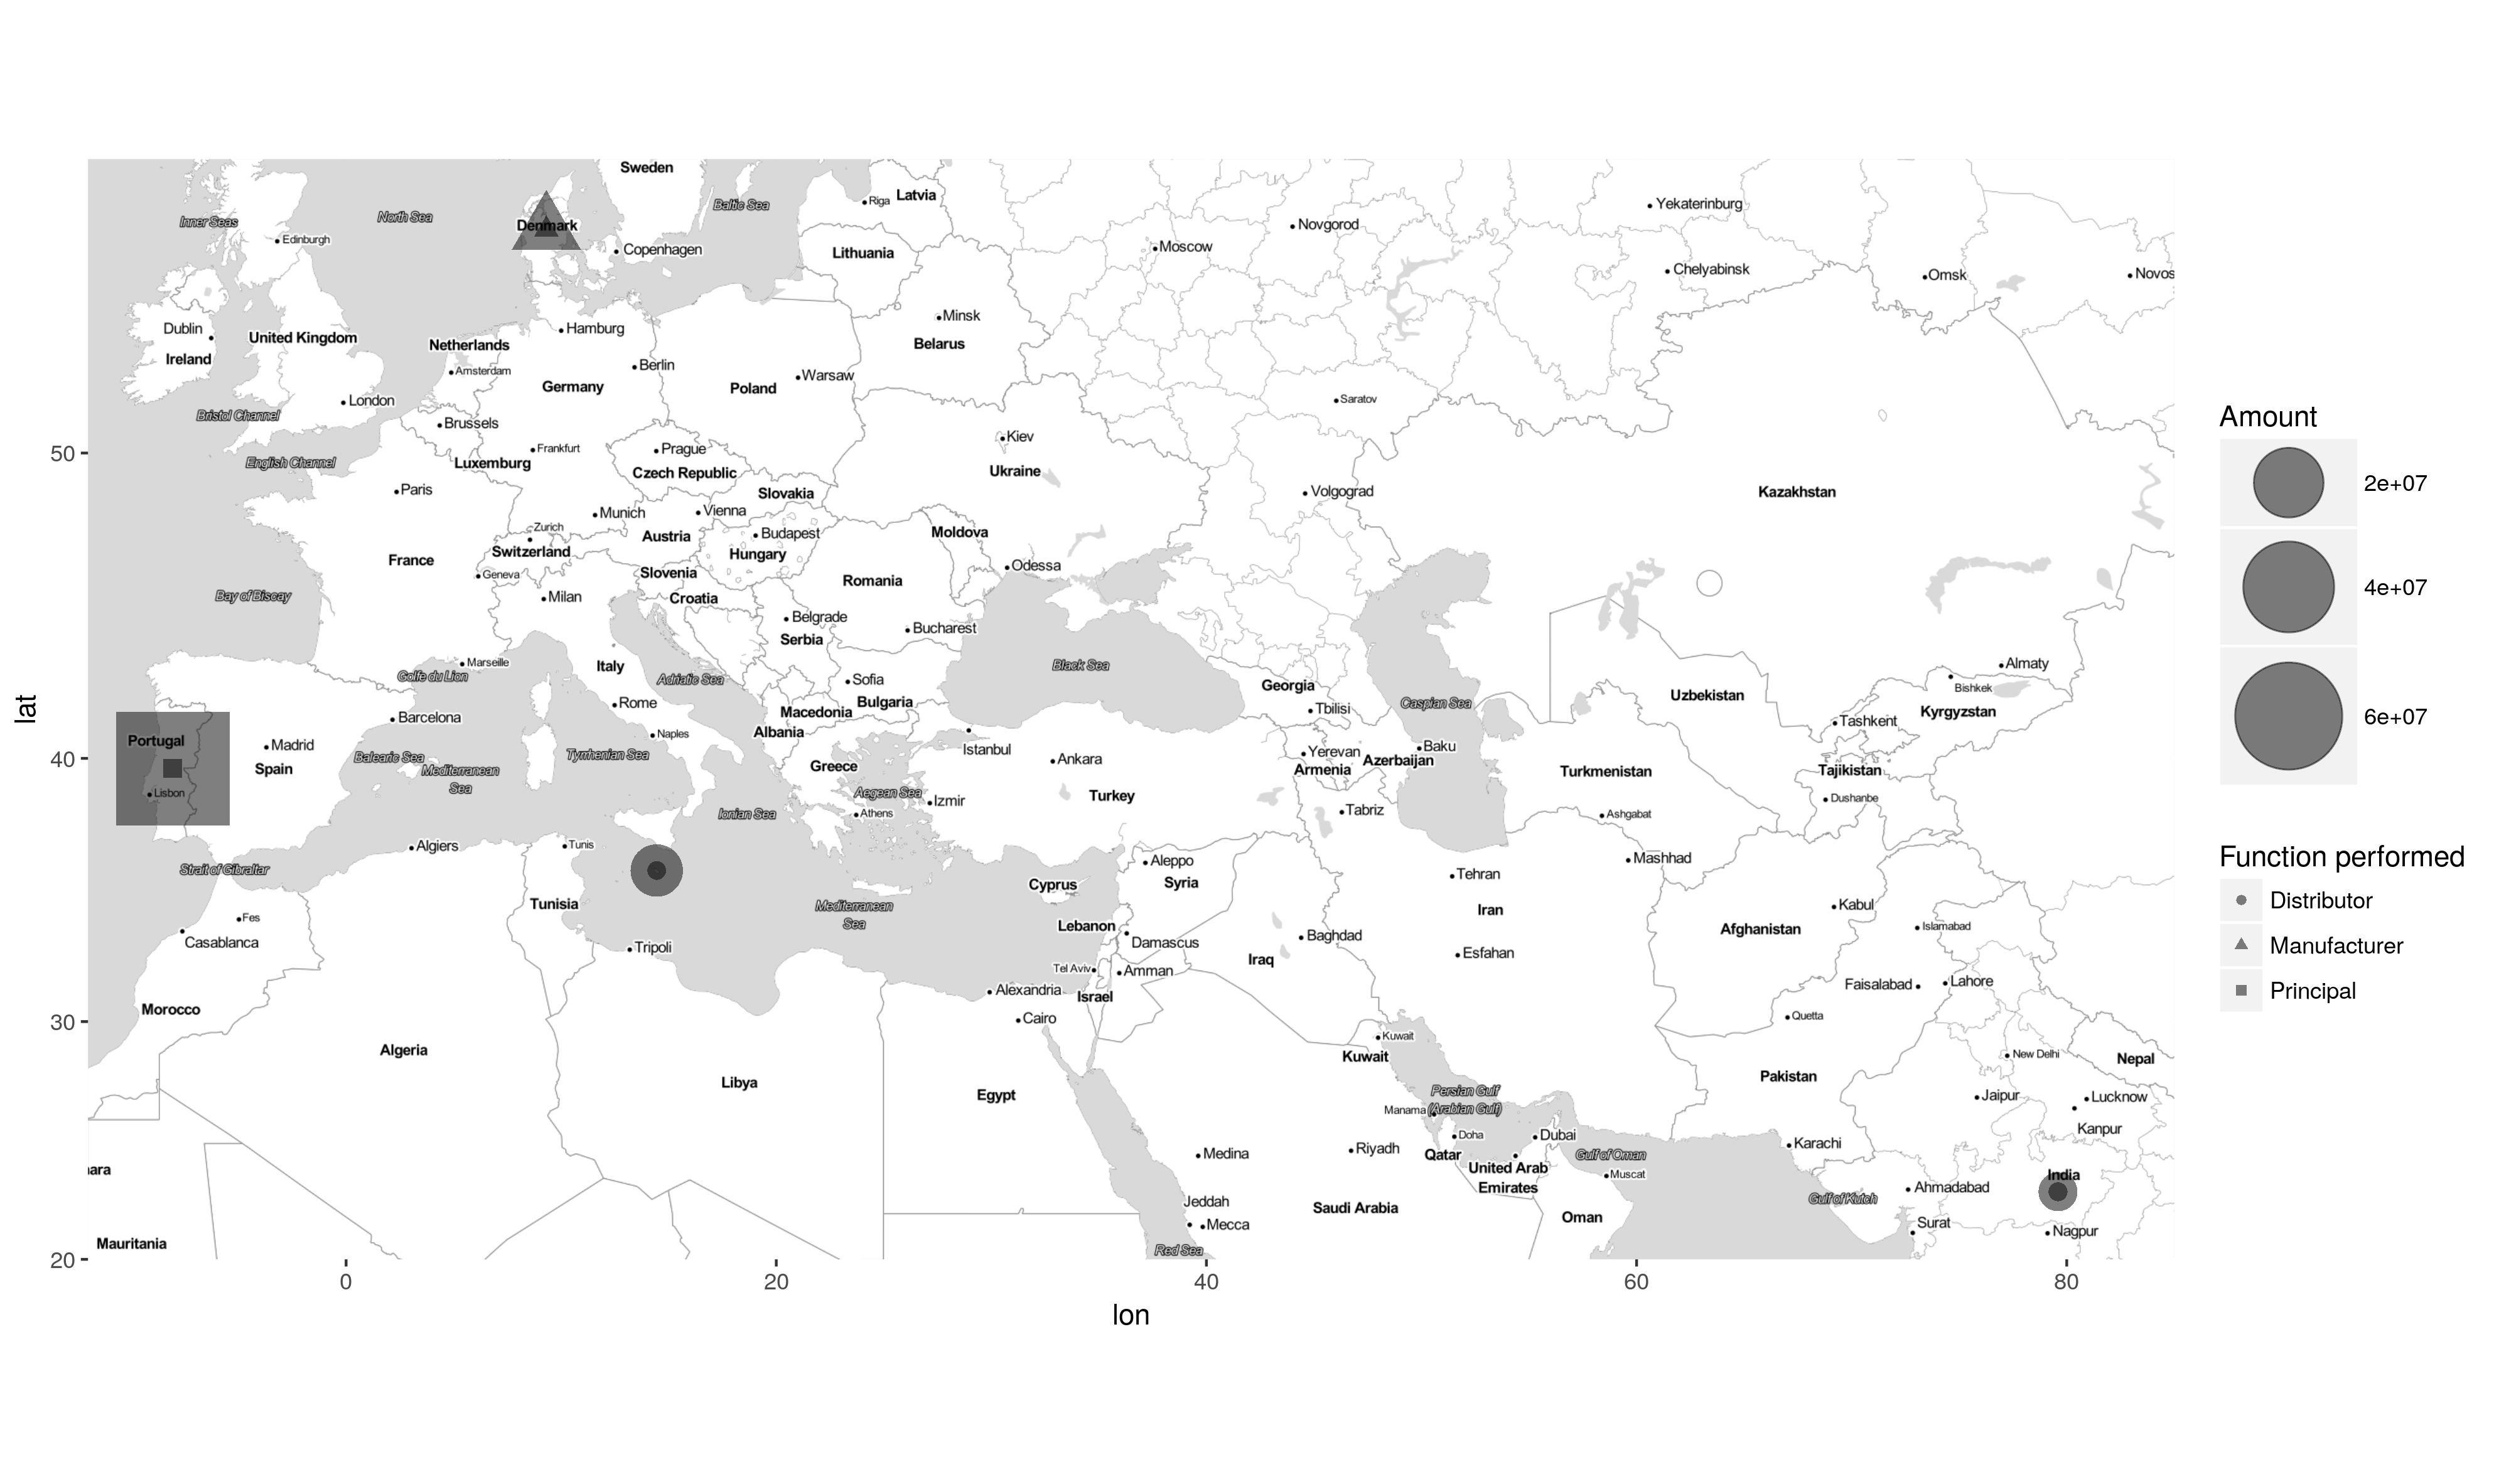
\includegraphics[width=0.8\linewidth]{allocation_map.png}
\captionof{figure}{\color{Green} Costs and revenues allocation according to to the model}
\end{center}\vspace{1cm}

The priority vector of the second model was more complex having a greater number of objectives, however such objectives may be divided into two big categories, namely customer oriented choices and green choices. 

\begin{wrapfigure}{l}{0.15\textwidth}
\begin{tabular}{l l}
\toprule
\textbf{Criteria} & \textbf{Weight} \\
\midrule
Transportation & 0.16 \\
Supporting Activities & 0.30 \\
Recycling Goal & 0.54 \\
Fulfill Demand & 0.16 \\
Cut Waste & 0.30 \\
Total & \textit{1.00} \\
\bottomrule
\end{tabular}
\captionof{table}{\color{Green} First model priority vector}
\end{wrapfigure}

The result achieved both the goal of cutting the overall waste made by the retail side constituted by disposed goods (NOCO) and fulfill the demand of goods by the costumers meaning that every retail point was reached. However the recycling goal was not fully achieved due to scarcity of disposed goods.
\\
\\
\\
\\
\begin{center}\vspace{1cm}
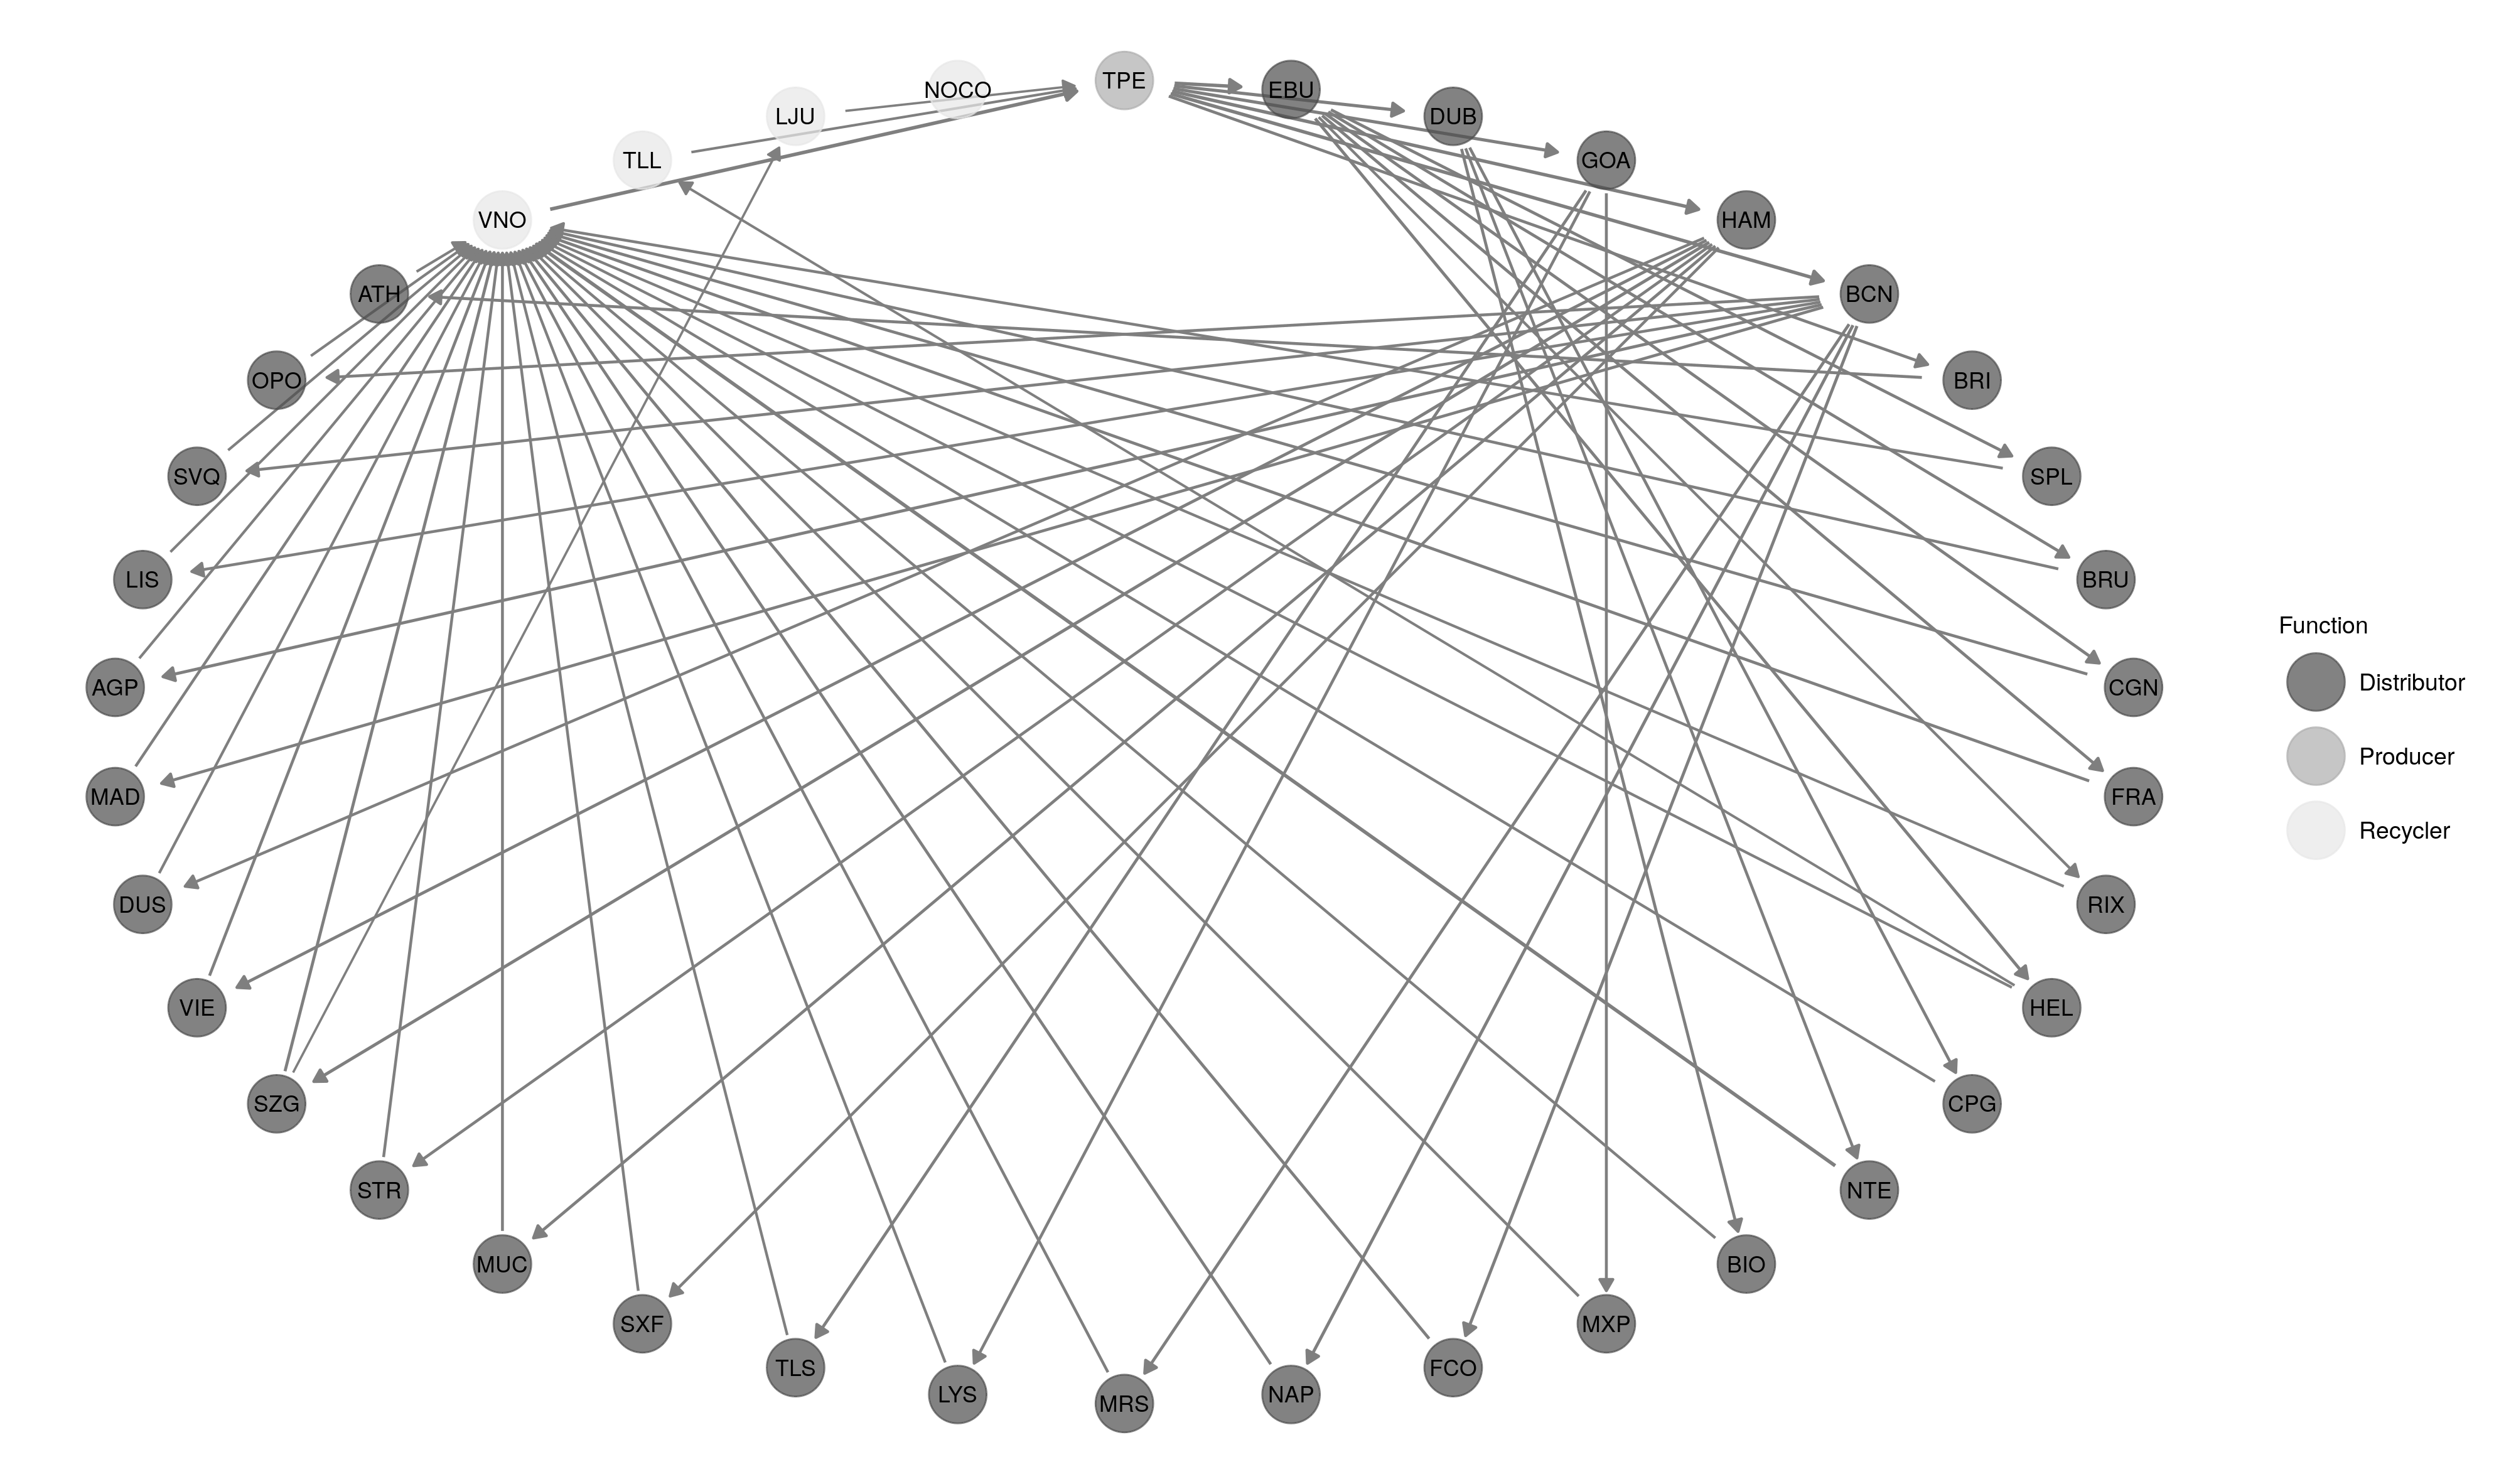
\includegraphics[width=0.8\linewidth]{network.png}
\captionof{figure}{\color{Green} Graphical interpretation of the Green Supply Chain network}
\end{center}\vspace{1cm}

\color{SaddleBrown} % SaddleBrown color for the conclusions to make them stand out

\section*{Conclusions}

\begin{itemize}
\item GP is a sound tool for decision making in multi national context;
\item GP is very versatile and can be implemented in almost any situation involving LP or MILP;
\item The software base to solve GP problems can scale with extreme simplicity;
\item The fields of research are not homogeneously developed leaving gray zones;
\item Operational related fields result in great expansion (as opposed to law related fields).
\end{itemize}

\color{DarkSlateGray}
\bibliographystyle{plain} % Plain referencing style
\bibliography{reference.bib}

\end{multicols}
\end{document}
